\documentclass[a4paper,10pt]{article}

\usepackage[utf8]{inputenc}             % Text encoding (accented characters).
\usepackage[english]{babel}             % Document language.
\usepackage[sfdefault]{roboto}          % Font used in the document.
\usepackage[T1]{fontenc}                % Hyphenation rule for accented characters (for the LaTeX compiler).

\usepackage{fancyhdr}                   % Adding headers and footers to each page of the document.
\usepackage{graphicx}                   % Addition of images into the document.
\usepackage{hyperref}                   % Creation of clickable links pointing to other parts of the document.
\usepackage{parskip}                    % Definable line breaks between each paragraph.

% Don't forget to change the "svgnames" option (colors defined on the RGB model, better for digital display)
% into "dvipsnames" option (based on the CMYK model, better for printing) in the script which converts each
% LaTeX document to printable format.

\usepackage[usenames,svgnames]{xcolor}                      % Text colouring.
\usepackage{verbatim}                                       % Paragraph layout.

\usepackage[document]{ragged2e}                             % Text justification.
\usepackage[a4paper,margin=1in,footskip=0.25in]{geometry}   % Document layout.


% -------------------------------------------------------------------------------------------------
% For more information and documentation on these LaTeX packages, please refer to the links below :

% inputenc  : https://www.ctan.org/pkg/inputenc
% babel     : https://www.ctan.org/pkg/babel
% roboto    : https://www.ctan.org/pkg/roboto
% fontenc   : https://www.ctan.org/pkg/fontenc

% fancyhdr  : https://www.ctan.org/pkg/fancyhdr
% graphicx  : https://www.ctan.org/pkg/graphicx
% hyperref  : https://www.ctan.org/pkg/hyperref
% parskip   : https://www.ctan.org/pkg/parskip

% xcolor    : https://www.ctan.org/pkg/xcolor
% verbatim  : https://www.ctan.org/pkg/verbatim

% ragged2e  : https://www.ctan.org/pkg/ragged2e
% geometry  : https://www.ctan.org/pkg/geometry


% -------------------------------------------------------------------------------------------------
% Writing the name of this file here in order to get it into the "docs_filename_hash.py" script and
% create a hash in order to better find its translated versions in the other languages folders.

% There is no need to copy this part in the translated versions of this document,
% since the aforementioned script only processes the English documentation files.

% Title for hashing (unused for this file) : "Bash-utils/docs/en/devtools/256-color-palette.tex"


% --------------------------------------------------------------------------------------------------
% List of defined colors (for the layout and for changing the theme for printing the documentation).

% Color definition               % Normal   | Printable     - Description

\definecolor{back}{HTML}{000000} % Black    | White         - Color of the document background.
\definecolor{case}{HTML}{fcff00} % Yellow                   - Color of the "case" conditions.
\definecolor{cmds}{HTML}{909090} % Gray                     - Color of the names of the system commands with their arguments.
\definecolor{cond}{HTML}{be480a} % Brick                    - Color of the "if" conditions.
\definecolor{func}{HTML}{800080} % Mauve                    - Color of the functions defined in each module of the Bash Utils framework.

\definecolor{loop}{HTML}{00ffff} % Cyan                     - Color of the loops.
\definecolor{main}{HTML}{8F00FF} % Violet                   - Color of the functions from the main script.
\definecolor{path}{HTML}{bfff00} % Lime                     - Color of the files and folders paths.
\definecolor{sec1}{HTML}{ff0000} % Red                      - Color of the main and first level titles.
\definecolor{sec2}{HTML}{00ff00} % Green                    - Color of the second level titles.

\definecolor{sec3}{HTML}{0060ff} % Blue                     - Color of the third level titles.
\definecolor{text}{HTML}{ffffff} % White    | Black         - Color of the normal text.
\definecolor{vars}{HTML}{FF7F00} % Orange                   - Color of the names of the parameters and the variables.


% ----------------------------------------------------------------
% Definition of the font and the background color of the document.

\fontfamily{Roboto}

\pagecolor{back}


% -----------------------------------------------
% Definition of the informations of the document.

\title{\color{sec1}Deciphering the mechanics behind the \textbf{\color{sec2}256-color-palette.sh} script}\color{text}
\author{Dimitri OBEID}
\pagestyle{fancy}

\pdfinfo{
  /Title    (Deciphering the mechanics behind the "256-color-palette.sh" script)
  /Author   (Dimitri OBEID)
  /Creator  (Dimitri OBEID)
  /Producer (Dimitri OBEID)
  /Subject  (Deciphering the mechanics behind the "256-color-palette.sh" script)
  /Keywords ()
}


% -----------------
% Paragraph layout.

\setlength{\parskip}{1em}


% --------------------------
% Beginning of the document.

\begin{document}
    \maketitle
    \newpage

    \hypertarget{contents}{}
    \tableofcontents
    \newpage

\color{sec1}
    \section{General presentation of the script}\color{text}

    \color{sec2}
    \subsection{Description of the script}\color{text}

    \begin{justify}
        This script displays each color code from the XTERM palette table on the terminal background in a 6 * 40 table, with the code corresponding to each color written in three digits in the foreground.
    \end{justify}

    % ------------

    % ----------------------

    % -----------------------------------------------

    \color{sec2}
    \subsection{How the script works}\color{text}

    \begin{justify}
        If the value "-h" or "--help" is passed as the first argument, a simple message summarizing the purpose of the script is displayed on the terminal, without its main code, written in the \textbf{\color{loop}for} loop, being executed.
    \end{justify}

    \begin{justify}
        This message will be displayed in the following languages, depending on the \textbf{\color{vars}\$LANG} environment variable. It will be displayed in English if the same variable does not contain the ISO 639-1 code for one of these languages:
    \end{justify}

    \begin{justify}
        \begin{itemize}
            \item German, English, Spanish, French, Indonesian, Portuguese, Russian, Ukrainian and Chinese.
        \end{itemize}

    \end{justify}


    \begin{justify}
    	\textbf{\color{loop}for} loop algorithm:

    	\textbf{\color{loop}While} the value of the \textbf{\color{vars}\$i} variable, initialized at 16 (value corresponding to the start number of the non-system color code range up to number 255 in the XTERM color table) is strictly less than 256, \textbf{\color{loop}then} :

        \begin{enumerate}
    	    \item The text background color is modified according to the color code corresponding to the value of the variable \textbf{\color{vars}\$i}, then the three-digit number corresponding to this same value is displayed.

    	    \setlength{\parskip}{1em}

    	    Here's how it works:

    	    \begin{itemize}
                \setlength{\parskip}{1em}

    	        \item \verb+'\e'+ : This is the escape character (ASCII code 27), which marks the beginning of any ANSI escape sequence.
    	        \item \textbf{48}: This is the code telling the Shell interpreter to change the text background color.

    	        \item \textbf{5}: This is the code indicating the use of a custom color index.

    	        \item \textbf{\color{vars}\${i}}: The value of this variable is used to define the XTERM color table number of the specific color to be displayed.

    	        \item \textbf{m}: This is the end code of the ANSI control sequence.
            \end{itemize}

    	    \setlength{\parskip}{1em}

    	    \item Text formatting is removed using the \textbf{\color{cmds}printf} \verb|'\e[0m'| command.

    	    \item
    	    {
                \textbf{\color{cond}If} the current color index is not the sixth of the current row, \textbf{\color{cond}then} a space is displayed to prepare the next iteration of the \textbf{\color{loop}for} loop via the \textbf{\color{cmds}printf} \verb|'\n'| command.

                \textbf{\color{cond}Else} a line break is made via the \textbf{\color{cmds}printf ' '} command to prepare a new row of six columns.
            }

    	    \item \textbf{\color{cond}End of the « if » condition}
    	\end{enumerate}

    	\textbf{\color{loop}End of the « for » loop}
    \end{justify}

    % ------------

    % ----------------------

    % -----------------------------------------------

    \newpage

    \color{sec2}
    \subsection{Displaying the XTERM palette table on the terminal}\color{text}

    \begin{justify}
    	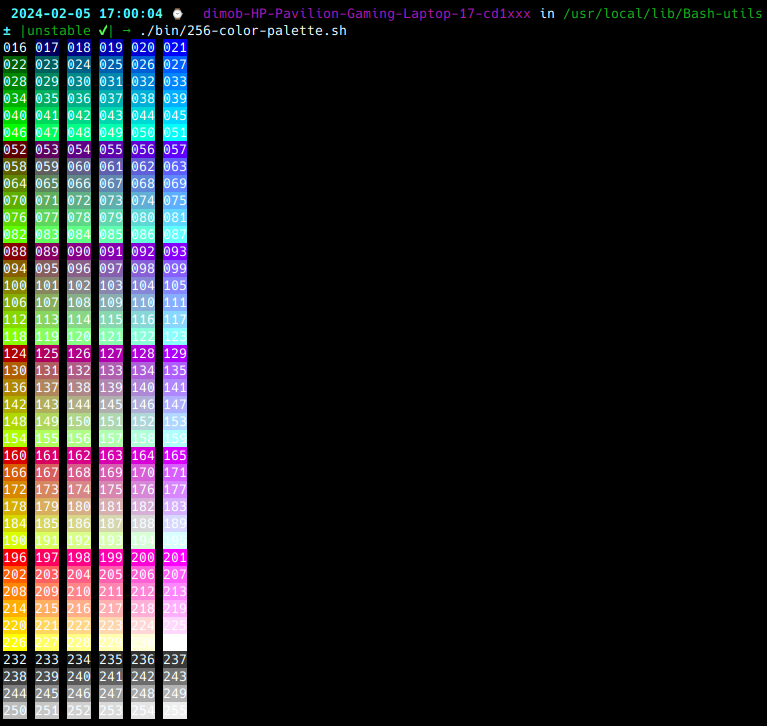
\includegraphics[scale=0.5884]{../../00 DATA/img/XTERM palette table.png}
    \end{justify}

	% ------------

    % ----------------------

    % -----------------------------------------------

    % /////////////////////////////////////////////////////////////////////////////////////////////// %

\end{document}
